\documentclass[titlepage,12pt,a4paper,times,oneside]{book}

\usepackage[utf8]{inputenc}
\usepackage[portuguese]{babel}
% substituir linha anterior por 
% \usepackage[english]{babel} 
% se o relatório for escrito na língua inglesa.
\usepackage[T1]{fontenc}
\usepackage{makeidx}
\usepackage{xspace}
\usepackage{graphicx,color,times}
\usepackage{fancyhdr}
% \usepackage{pxfonts}
% \usepackage{times}
% \usepackage{mathptm}
% \usepackage{amssymb}
% \usepackage{amsfonts}
\usepackage{amsmath}
\usepackage{latexsym}
\usepackage[printonlyused]{acronym}
\usepackage{float}
\usepackage{listings}
\usepackage{tocbibind}
\usepackage{wrapfig}
% \usepackage{natbib}
\usepackage{hyperref}
% \usepackage{glossaries}
% \makeglossaries

\usepackage{minted}
\usepackage{paralist}
\usepackage{enumitem}
\usepackage{booktabs}
\usepackage{amssymb}
\usepackage{calc}
\usepackage{array}
\usepackage{color}
\usepackage{colortbl}
% \usepackage{biblatex}

% \renewcommand{\ttdefault}{phv}

\pagestyle{fancy}
\renewcommand{\chaptermark}[1]{\markboth{#1}{}}
\renewcommand{\sectionmark}[1]{\markright{\thesection\ #1}}
\fancyhf{} \fancyhead[LE,RO]{\bfseries\thepage}
\fancyhead[LO]{\bfseries\rightmark}
\fancyhead[RE]{\bfseries\leftmark}
\renewcommand{\headrulewidth}{0.5pt}
\renewcommand{\footrulewidth}{0pt}
\addtolength{\headheight}{0.5pt}
\setlength{\marginparsep}{0cm}
\setlength{\marginparwidth}{0cm}
\setlength{\marginparpush}{0cm}
\addtolength{\hoffset}{-1.0cm}
\addtolength{\oddsidemargin}{\evensidemargin}
\addtolength{\oddsidemargin}{0.5cm}
\addtolength{\evensidemargin}{-0.5cm}


% NEW COLORS
\definecolor{dark}{gray}{0.25}
\definecolor{lgray}{gray}{0.9}
\definecolor{dkblue}{rgb}{0,0.13,0.4}
\definecolor{dkgreen}{rgb}{0,0.6,0}
\definecolor{gray}{rgb}{0.5,0.5,0.5}
\definecolor{mauve}{rgb}{0.58,0,0.82}

\lstset{ %
  language=C,                    basicstyle=\footnotesize,
  numbers=none,                  numberstyle=\tiny\color{gray}, 
  stepnumber=1,                  numbersep=5pt,
  backgroundcolor=\color{white}, showspaces=false,
  showstringspaces=false,        showtabs=false,
  frame=single,                  rulecolor=\color{black},
  tabsize=2,                     captionpos=b,
  breaklines=true,               breakatwhitespace=false,
  title=\lstname,                keywordstyle=\color{blue},
  commentstyle=\color{dkgreen},  stringstyle=\color{mauve},
  escapeinside={\%*}{*)},        morekeywords={*},
  belowskip=0cm
}

\renewcommand{\listingscaption}{Excerto de Código}
\renewcommand{\listoflistingscaption}{Lista de Excertos de Código}% 

\graphicspath{{./img/}}
\newcommand{\usecasescale}{0.5}

\newcommand{\theteam}{C-Team}
\newcommand{\theapp}{Challenge Accepted}
\newcommand{\groupname}{{\itshape\theteam}}
\newcommand{\appname}{{\itshape\theapp}}

\newcommand{\famousquote}[2]{
	\begin{quote}
		\rule{\textwidth-2\leftmargin}{0.4pt}
		{\itshape #1}
		\vspace{-12pt}
		\begin{flushright}
			\textasciitilde~#2
		\end{flushright}
		\vspace{-20pt}
		\rule{\textwidth-2\leftmargin}{0.4pt}
	\end{quote}
}

% \setlist{nosep}


\begin{document}

\thispagestyle{empty}
\setcounter{page}{-1}

\begin{center}
\begin{Huge}
\textbf{Universidade da Beira Interior}
\end{Huge}
\end{center}

\begin{center}
\begin{Huge}
Departamento de Informática
\end{Huge}
\end{center}

\vspace{0,07cm}
\begin{figure}[!htb]
\centering

\includegraphics[width=191pt]{ubi-fe-di.png}
\end{figure}

\vspace{0.5cm}
\begin{center}
\begin{Large}
\textbf{\theteam: \appname}
\end{Large}
\end{center}

\vspace{0.5cm}
\begin{center}
\begin{normalsize}
\begin{large}
Elaborado por:
\end{large}
\end{normalsize}
\end{center}

\vspace{0.2cm}
\begin{center}
\begin{large}
\begin{tabular}{>{\bfseries}r @{~~---~~} >{\bfseries}l}
	38950 & Diogo José Real Lavareda    \\
	39392 & Joana Elias Almeida         \\
	41266 & Diogo Castanheira Simões    \\
	41358 & Beatriz Tavares da Costa    \\
	41381 & Igor Cordeiro Bordalo Nunes
\end{tabular}
\end{large}
\end{center}

\vspace{0,5cm}
\begin{center}
\begin{normalsize}
\begin{large}
Orientador:
\end{large}
\end{normalsize}
\end{center}

\vspace{0.2cm}
\begin{center}
\begin{large}
\textbf{Professor Doutor Pedro Ricardo Morais Inácio}
\end{large}
\end{center}

\vspace{0.5cm}
\begin{center}
\begin{normalsize}
%\today
22 de maio de 2021
\end{normalsize}
\end{center}

\clearpage{\thispagestyle{empty}\cleardoublepage}

\frontmatter

\chapter*{Resumo}
\label{chap:resumo}

A criptografia é célebre pelas suas práticas e técnicas de comunicação segura, contudo a mesma não é usada apenas na iminência de inimigos. Sendo que na era atual a criptografia já se encontra um pouco por todo o nosso quotidiano, porque não usar as suas ferramentas para o nosso lazer?

Sendo este um tema ligado à criptografia, escolhemos abordá-lo de forma informativa e acessível para que o utilizador tenha uma experiência segura ao desfrutar do seu tempo.

Nesta medida, foi criada uma plataforma denominada \appname, que oferece a todos os seus utilizadores a oportunidade de desenvolver desafios criptográficos e também de resolver os deixados por outros utilizadores.



%\clearpage{\thispagestyle{empty}\cleardoublepage}


\tableofcontents

%\clearpage{\thispagestyle{empty}\cleardoublepage}

\listoffigures

% Se não existirem tabelas, comentar as seguintes linhas
%\clearpage{\thispagestyle{empty}\cleardoublepage}
\listoftables

% Se existirem trechos de código, descomentar as seguintes linhas
% \clearpage{\thispagestyle{empty}\cleardoublepage}
\listoflistings
\addcontentsline{toc}{chapter}{\listoflistingscaption}

%\clearpage{\thispagestyle{empty}\cleardoublepage}
\chapter*{Acrónimos}
\label{ch::acro}

\begin{acronym}[CFIUTE]
	\acro{API}{\textit{Application Programming Interface}}
	\acro{APK}{\textit{Android Application Package}}
	\acro{ARGB}{\textit{Alpha-Red-Green-Blue}}
	\acro{CFIUTE}{Centro de Formação Interação UBI Tecido Empresarial}
	\acro{FQDN}{\emph{Fully Qualified Domain Name}}
	\acro{eduroam}{\emph{Education Roaming}}
	\acro{HTML}{\textit{Hypertext Markup Language}}
	\acro{JDK}{\textit{Java Development Kit}}
	\acro{MVC}{\textit{Model-View-Controller}}
	\acro{RSA}{\emph{Rivest-Shamir-Adleman}}
	\acro{SMTP}{\textit{Simple Mail Transfer Protocol}}
	\acro{SSL}{\emph{Secure Sockets Layer}}
	\acro{SWOT}{\textit{Strength, Weakness, Opportunity, and Threat Analysis}}
	\acro{TaC}{\textit{Together Against Cybercrime}}
	\acro{TI}{Tecnologias de Informação}
	\acro{TUI}{\emph{Text-based User Interface}}
	\acro{UC}{Unidade Curricular}
	\acro{UI}{\textit{User Interface}}
	\acro{URI}{\textit{Uniform Resource Identifier}}
	\acro{XML}{\textit{Extended Markup Language}}
\end{acronym}

% \clearpage{\pagestyle{empty}\cleardoublepage}
% \chapter*{Glossário}
\makeglossaries

\newglossaryentry{.NET Framework}
{
  name={.NET Framework},
  description={É uma plataforma para desenvolvimento e funcionamento de aplicações desenvolvida pela Microsoft.}
}

\newglossaryentry{ASP.NET}
{
  name={ASP .Net},
  description={É uma plataforma da Microsoft para o desenvolvimento de aplicações Web e é o sucessor da tecnologia ASP.}
}

\newglossaryentry{CS}
{
  name={C\#},
  description={Lê-se \textit{C Sharp} e é uma linguagem de programação orientada a objectos, desenvolvida pela Microsoft, inicialmente para a plataforma .NET. O C\# é inspirado na junção entre as linguagens C++ e Java.}
}


\newglossaryentry{Java}
{
  name={JAVA},
  description={É uma linguagem de programação orientada a objectos, desenvolvida pela Sun Microsystems na década de 90. Hoje pertence à empresa Oracle.}
}


\newglossaryentry{OpenDMTP}
{
  name={OpenDMTP},
  description={\textit{Open Device Monitoring and Tracking Protocol} é um protocolo e uma \textit{framework} abertos que permite a comunicação bidireccional entre servidores e clientes através da internet.}
}


\newglossaryentry{OpenGTS}
{
  name={Open GTS},
  description={É o primeiro projecto \textit{Open Source} \textit{Web-Based} para controlo de frotas por GPS.}
}


\newglossaryentry{VS2010}
{
  name={Visual Studio 2010},
  description={\textit{Microsoft Visual Studio 2010} é um sistema de desenvolvimento desenvolvido pela Microsoft e é dedicado ao Framework .NET, que contem um conjunto de ferramentas de desenvolvimento projectadas para auxiliar os programadores a enfrentarem desafios complexos.}
}


\newglossaryentry{WebS}
{
	name={Web Service},
	description={Web services são aplicações modulares auto-descritas e auto-contidas, que permitem a integração de sistemas e a comunicação entre aplicações de diferentes tipos.}
}


\newglossaryentry{WebBased}
{
	name={Web Based},
	description={Aplicação desenvolvida para a Web.}
}

\newglossaryentry{Roaming}
{
	name={Roaming},
	description={Define a possibilidade de um utilizador de uma determinada rede obter rede/conecção fora da área geográfica onde foi registado.}
}


\newglossaryentry{Smartphone}
{
	name={Smartphone},
	description={Smartphone é um telefone móvel que contem muitas das principais tecnologias de comunicação e serviços que existem nos computadores pessoais, como acesso a e-mails, serviços de mensagens instantâneas, internet, GPS, entre outros.}
}

\newglossaryentry{TCPIP}
{
	name={TCP/IP},
	description={É um conjunto de protocolos de comunicação entre computadores ligados rede. O nome TCP/IP surge da união entre dois protocolos: o TCP (Transmission Control Protocol) e o protocolo IP (Internet Protocol).}
}

\newglossaryentry{Firewall}
{
	name={Firewall},
	description={É o nome criado para definir um dispositivo para uma rede de computadores que tem como objectivo criar uma política de segurança num determinado ponto de controlo da rede.}
}

\newglossaryentry{JavaScript}
{
	name={JavaScript},
	description={É uma linguagem de programação baseada na linguagem de programação ECMAScript. Actualmente é a linguagem de programação mais utilizada em \textit{``Client-Side''} nos \textit{browsers}.}
}

\newglossaryentry{Flash}
{
	name={Flash},
	description={Desenvolvido pela Macromedia, o Flash é um software utilizado para criação de animações interactivas que funcionam incorporadas em \textit{Browsers}, \textit{Desktop}, \textit{Smartphones}, \textit{Tablets}, e Televisores.}
}


\newglossaryentry{StoredProcedure}
{
	name={Stored Procedure },
	description={É o nome dado a um conjunto de comandos numa base de dados de forma a simplificar a sua utilização.}
}

\newglossaryentry{SQLS}
{
	name={SQL Server 2008},
	description={É um sistema de gestão de base de dados relacional criado pela Microsoft.}
}

\newglossaryentry{Firm}
{
	name={Firmware},
	description={É o conjunto de instruções operacionais programadas directamente no \textit{hardware} de um equipamento electrónico.}
}

\newglossaryentry{browser}
{
	name={Browser},
	description={É um programa de computador que possibilita aos utilizadores uma interacção com documentos virtuais da Internet, também conhecidos como páginas Web.}
}



%\clearpage{\thispagestyle{empty}\cleardoublepage}

\mainmatter
\acresetall
\chapter{Introdução}
\label{chap:intro}

\section{Descrição da proposta}
\label{sec::intro:descricao}

A criptografia é uma das estratégias mais importantes para garantir segurança de dados. Atualmente enfrentamos uma era de globalização com ataque a sistemas para roubo de informações privilegiadas, com o intuito de proveito próprio ou venda das mesmas a terceiros, entre outros fins.

Sendo uma temática tão importante e atual, pretende-se levar a mesma ao público geral e poder transmitir a ``magia'' dos desafios criptográficos.

A aplicação \appname~tem como objetivos permitir aos utilizadores registados publicar e resolver desafios criptográficos, bem como tornar-se numa ferramenta educativa na área da criptografia.

% O projeto foi proposto pelo Professor Doutor Pedro Ricardo Morais Inácio no âmbito da cadeira Segurança Informática, lecionada pelo mesmo.


\section{Constituição do grupo}
\label{sec::intro:grupo}

O presente projeto foi realizado pela equipa \textit{C-Team}, constituída pelos elementos listados na Tabela \ref{tab::c-team}.

\begin{table}[!h]
	\centering
	\begin{tabular}{c l >{\itshape}l}
		\toprule
		\textbf{N\textordmasculine} & \textbf{Nome} & \normalfont\textbf{Alcunha} \\
		\midrule
		38950 & Diogo José Real Lavareda    & Lavareda \\
		39392 & Joana Elias Almeida         & Joaninha \\
		41266 & Diogo Castanheira Simões    & Ash      \\
		41358 & Beatriz Tavares da Costa    & Bea      \\
		41381 & Igor Cordeiro Bordalo Nunes & Etileno  \\
		\bottomrule
	\end{tabular}
	\caption[Constituição da equipa \textit{C-Team}]{Constituição da equipa \textit{C-Team}.}
	\label{tab::c-team}
\end{table}



\section{Organização do Documento}
\label{sec::intro:organizacao}

De modo a refletir o projeto realizado, este relatório encontra-se estruturado em cinco capítulos, nomeadamente:

\begin{enumerate}
\item No primeiro capítulo --- \textbf{Introdução} --- são apresentados o projeto, os seus objetivos, a equipa desenvolvedora e a respetiva organização do relatório.

\item No segundo capítulo --- \textbf{Engenharia de Software} --- são elaborados os diagramas de casos de uso da aplicação que orientam a respetiva implementação.

\item No terceiro capítulo --- \textbf{Implementação} --- são descritas as escolhas e os detalhes de implementação da aplicação, bem como as tecnologias utilizadas durante o seu desenvolvimento.

\item No quarto capítulo --- \textbf{Reflexão Crítica e Problemas Encontrados} --- são indicados os objetivos alcançados, quais as tarefas realizadas por cada membro do grupo, assim como são expostos os problemas enfrentados e é feita uma reflexão crítica sobre o trabalho.

\item No quinto capítulo --- \textbf{Conclusões e Trabalho Futuro} --- são analisados os conhecimentos adquiridos ao longo do desenvolvimento do projeto e, em contrapartida, o que não se conseguiu alcançar e que poderá ser explorado futuramente.
\end{enumerate}

%\clearpage{\thispagestyle{empty}\cleardoublepage}
\chapter{Engenharia de Software}
\label{ch::engsoft}


\section{Introdução}
\label{sec::engsoft:intro}

% Um projeto de sucesso envolve uma preparação prévia exímia.
A plataforma \appname~desenvolvida pela \groupname~não foi exceção. Foram delineados antecipadamente vários pontos fulcrais, nomeadamente:

%TODO: I'm here <--

\begin{itemize}
    \item Ferramentas e tecnologias (Secção \ref{sec::engsoft:tecnologia}): perante uma equipa de 5 pessoas, foi vital determinar quais as tecnologias a utilizar não só para implementar a aplicação mas também para gerir o trabalho paralelo que iria decorrer;
    \item Requisitos funcionais e não-funcionais (Secção \ref{sec::engsoft:requisitos}): a aplicação deve cumprir uma série de requisitos a fim de poder alcançar os objetivos propostos;
    \item Diagramas de casos de uso (Secção \ref{sec::engsoft:casos-uso}): a fim de se perceber as atividades a desenhar e o respetivo código-fonte que as interliga, diferentes casos de uso foram estudados;
    \item Diagrama de atividades (Secção \ref{sec::engsoft:casos-uso}): este diagrama resume o fluxo de funcionamento da aplicação.
\end{itemize}


\section{Ferramentas e tecnologias utilizadas}
\label{sec::engsoft:tecnologia}

As ferramentas utilizadas no âmbito da realização do projeto, sumariadas na Tabela \ref{tab::ferramentas}, visam três componentes essenciais na sua gestão: 1) linguagem de programação, 2) servidor, 3) administração bd, 4) relatório, 5) controlo de versões.


\begin{table}[!htbp]
    \centering
    \begin{tabular}{p{1cm} l l}
        \toprule
        & {\itshape\bfseries Software} & {\bfseries Versão} \\
        \midrule
        \multicolumn{3}{l}{\bfseries Linguagem de Programação} \\
        & \textit{Python} & 3.8.0 \\
        \midrule
        \multicolumn{3}{l}{\bfseries Servidor} \\
        & \textit{Microsoft Windows Server} & 2019 \\
        & \textit{MariaDB} & 10.4.18 \\
        \midrule
        \multicolumn{3}{l}{\bfseries Administração BD} \\
        & \textit{DBeaver} & 21.0.5 \\
        \midrule
        \multicolumn{3}{l}{\bfseries Relatório} \\
        & \textit{Overleaf} & \\
        \midrule
        \multicolumn{3}{l}{\bfseries Controlo de versões} \\
        & \textit{git} & 2.17.1 \\
        & \textit{GitKraken} & 7.6.1  \\
        \midrule
        \bottomrule
    \end{tabular}
    \caption[Ferramentas utilizadas]{Ferramentas e tecnologias utilizadas, organizadas por categoria.}
    \label{tab::ferramentas}
\end{table}



\section{Requisitos}
\label{sec::engsoft:requisitos}

De forma a ir de encontro aos objetivos propostos do projeto (Secção \ref{sec::intro:descricao}), uma série de requisitos funcionais e não-funcionais foi delineada.

\subsection{Requisitos funcionais}
\label{ssec::engsoft:requisitos:funcionais}

A plataforma deve:

\begin{enumerate}
    \item Possuir um ecrã de boas-vindas e instruções de uso do sistema;
    \item Ter um ecrã de registo e \emph{login} de utilizadores;
    \item Ter uma \textit{homepage} com acesso direto às seguintes funcionalidades:
    \begin{enumerate}
        \item resolução de desafios disponíveis,
        \item propor desafios,
        \item pedir ajuda,
        \item \textit{scoreboard} dos utilizadores,
    \end{enumerate}
    \item Permitir responder a desafios;
    \item Permitir submeter dois tipos de desafios, em que um é de decifra de mensagem e outro de descoberta de mensagem.
\end{enumerate}


\subsection{Requisitos não-funcionais}
\label{ssec::engsoft:requisitos:nao-funcionais}

A plataforma deve:

\begin{enumerate}
    \item Permitir apenas uma tentiva a cada 15 segundos para os desafios cifrados;
    \item Usar assinaturas digitais \ac{RSA};
    \item Ter uma interface gráfica minimalista e (\textit{user-friendly});
    \item Ser segura em termos do armazenamento dos dados na base de dados (se possível cifrar os dados guardados duplamente no caso dos desafios).
\end{enumerate}


\section{Casos de Uso}
\label{sec::engsoft:casos-uso}

Para a plataforma \emph{CHALLENGE-ACCEPTED}, foram identificados os seguintes casos de uso:
\begin{enumerate}
    \item Processo de Registo e \emph{Login} (Figura \ref{fig::casos-uso-regis});
    \item \textit{Homepage} (Figura \ref{fig::casos-uso-homepage});
    \item Processo de propor desafio e cifra de mensagem (Figura \ref{fig::casos-uso-propdesafio});
    \item Processo de responder a desafios (Figura \ref{fig::casos-uso-repdesafio});
    \item Processo de propor desafios do tipo valor de hash (Figura \ref{fig::casos-uso-hash});
\end{enumerate}

Os diagramas foram elaborados com recurso ao serviço \textit{Visual Paradigm}.

\begin{figure}[!htbp]
    \centering
    %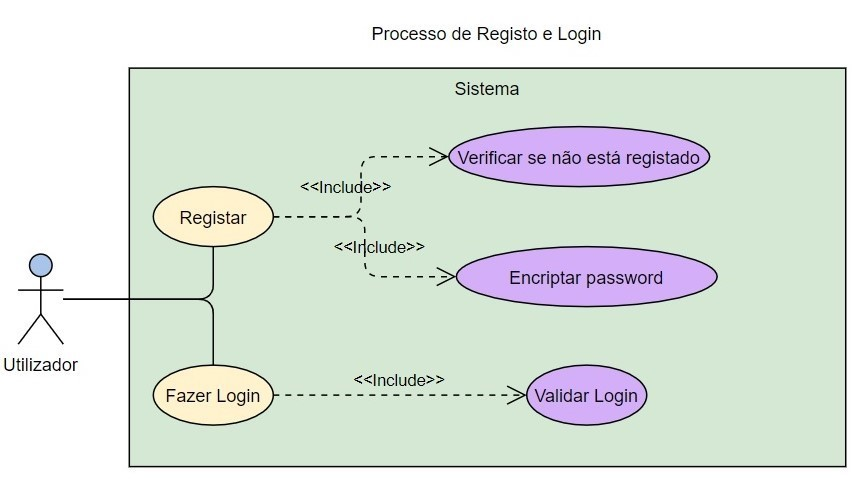
\includegraphics[scale=0.8]{Processo_Registo_Login.jpg}
    \caption[Diagrama de casos de uso: processo de registo e \emph{Login}]{Diagrama de casos de uso: processo de registo e \emph{Login}}
    \label{fig::casos-uso-regis}
\end{figure}

\begin{figure}[!htbp]
    \centering
    %\includegraphics[scale=0.8]{uso-homepage}
    \caption[Diagrama de casos de uso: \emph{homepage}]{Diagrama de casos de uso: \emph{homepage}.}
    \label{fig::casos-uso-homepage}
\end{figure}

\begin{figure}[!htbp]
    \centering
    %\includegraphics[scale=0.8]{uso-propdesafio}
    \caption[Diagrama de casos de uso: processo de propor desafio e cifra de mensagem]{Diagrama de casos de uso: processo de propor desafio e cifra de mensagem.}
    \label{fig::casos-uso-propdesafio}
\end{figure}

\begin{figure}[!htbp]
    \centering
    %\includegraphics[scale=0.8]{uso-repdesafio}
    \caption[Diagrama de casos de uso: processo de responder a desafios]{Diagrama de casos de uso: processo de responder a desafios.}
    \label{fig::casos-uso-repdesafio}
\end{figure}

\begin{figure}[!htbp]
    \centering
    %\includegraphics[scale=0.8]{uso-hash}
    \caption[Diagrama de casos de uso: processo de propor desafios do tipo valor de hash]{Diagrama de casos de uso: processo de propor desafios do tipo valor de hash.}
    \label{fig::casos-uso-hash}
\end{figure}

\section{Diagrama do sistema}
\label{sec::engsoft:diagrama-sistema}

\begin{figure}[!htbp]
    \centering
    %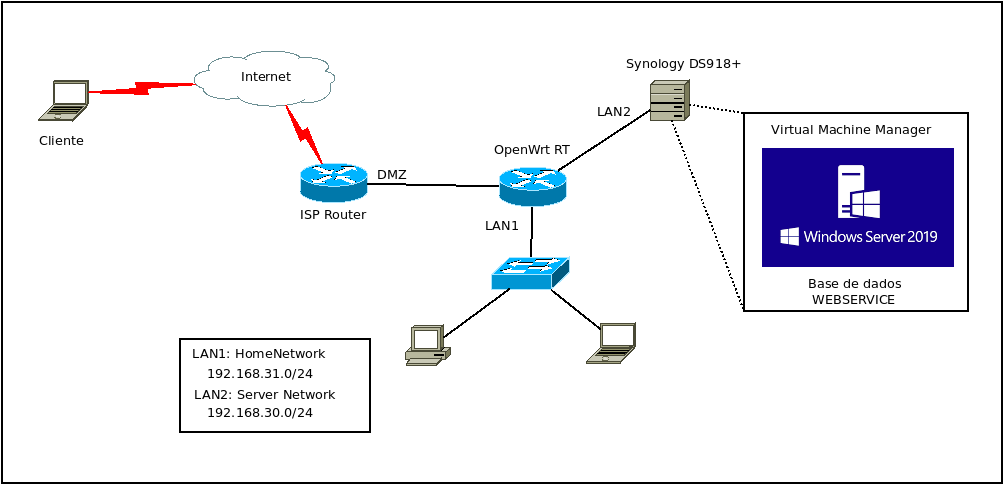
\includegraphics[scale=0.37]{DiagramaIdeal.png}
    \caption[Diagrama da arquitetura do sistema]{Diagrama da arquitetura do sistema}
    \label{fig::diagrama-sistema}
\end{figure}


\section{Conclusões}
\label{sec::engsoft:conclusao}

Na posse de um plano delineado segundo as práticas comuns da área da Engenharia de \textit{Software}, segue-se a fase de implementação, a qual deve seguir escrupulosamente os requisitos determinados e tem por base os casos de uso estudados. Por fim, o fluxo da aplicação deverá seguir o diagrama de atividades obtido por esta fase de estudo.


%\clearpage{\thispagestyle{empty}\cleardoublepage}
\chapter{Implementação}
% OU \chapter{Trabalhos Relacionados}
% OU \chapter{Engenharia de Software}
% OU \chapter{Tecnologias e Ferramentas Utilizadas}
\label{ch::implementacao}

\section{Introdução}
\label{sec::implementacao:intro}

A fase de implementação envolveu a execução paralela de diferentes tarefas pelos vários elementos da equipa. Este Capítulo aborda em particular os seguintes aspetos desta fase do projeto:

\begin{itemize}
    \item Interface (Secção \ref{sec::implementacao:tui}): aborda as escolhas feitas na construção da \acf{TUI};
    \item Escolhas de implementação (Secção \ref{sec::implementacao:escolhas}): explica as decisões feitas durante a implementação do código-fonte;
    \item Detalhes de implementação (Secção \ref{sec::implementacao:detalhes}): explora os detalhes mais importantes do código-fonte.
\end{itemize}

Adicionalmente, são descritos o malual de instalação (Secção \ref{sec::implementacao:maninstall}) e o manual de utilização (Secção \ref{sec::implementacao:manuser}).


\section{Interface --- \ac{TUI}}
\label{sec::implementacao:tui}

Para a interface foram analisadas primeiramente duas opções existentes em bibliotecas do \textit{Python}: \textit{npyscreen} e \textit{picotui}. Contudo, ambas revelaram ter uma curva de aprendizagem que não compensaria face às restantes tarefas a realizar na elaboração do projeto.

Neste sentido, a \ac{TUI} segue uma filosofia minimalista e clássica de leitura de dados introduzidos por parte do utilizador, incluindo as opções dos menus para navegação.

Não obstante, a aplicação segue um código de cores para diferenciar os diferentes tipos de informação dados ao utilizador (Tabela \ref{tab::cores}).

\begin{table}[!htbp]
    \centering
    \begin{tabular}{>{\itshape}l l p{1cm}}
        \toprule
        \normalfont{\bfseries Cor} & \normalfont{\bfseries Utilização} & \\
        \midrule
        Vermelho & Mensagem de erro (\textit{error})       & \cellcolor[rgb]{1., 0., 0.} \\
        Amarelo  & Mensagem de aviso (\textit{warning})    & \cellcolor[rgb]{0.941, 0.886, 0.23} \\
        Verde    & Mensagem de sucesso (\textit{success})  & \cellcolor[rgb]{0., 1., 0.} \\
        Ciano    & Informação da aplicação (\textit{info}) & \cellcolor[rgb]{0.239, 0.843, 0.941} \\
        Cinza    & Mensagens de \textit{debug} (reservado) & \cellcolor[rgb]{0.4, 0.4, 0.4} \\
        \bottomrule
    \end{tabular}
    \caption[Cores por tipo de mensagem]{Palete de cores utilizada por cada tipo de mensagem dada ao utilizador.}
    \label{tab::cores}
\end{table}


\section{Escolhas de Implementação}
\label{sec::implementacao:escolhas}

De entre as escolhas efetuadas durante a implementação da aplicação, três em
particular destacam-se:

\begin{itemize}
    \item \textbf{\textit{Python}:}\\
        A seleção da linguagem de programação teve como critérios ser de alto nível, fornecer bibliotecas atualizadas de segurança e criptografia, e disponibilizar \textit{frameworks} acessíveis para a criação de um \textit{webservice}. A escolha final recaiu, portanto, na linguagem \textit{Python}.
    
    \item \textbf{\textit{MariaDB}:}\\
        Uma vez que o grupo se encontra familiarizado com bases de dados relacionais, e sendo este um modelo adequado para os dados a guardar, optou-se por uma solução \textit{open-source}, estável, atualizada e com reputação no mundo profissional: \textit{MariaDB}.
    
    \item \textbf{\textit{Flask}:}\\
        Após a escolha da linguagem \textit{Python}, a \textit{framework} que rapidamente se destacou para a criação do \textit{webservice} foi o \textit{Flask}. Destaca-se o facto da curva de aprendizagem desta ferramenta ser curta.
\end{itemize}


\section{Detalhes de Implementação}
\label{sec::implementacao:detalhes}

% TODO: Detalhes

%Porquanto a implementação no seu todo desse facilmente origem a um vasto documento técnico, três situações destacaram-se:

\subsection{Navegação}
\label{ssec::implementacao:detalhes:nav}

A navegação é feita com menus, os quais são objetos instanciados da classe \verb|Menu|, criada para este projeto. Esta classe permite fazer a gestão automatizada de menus, sendo uma função invocada quando uma dada opção válida do menu é selecionada.

Tal permite tirar partido da \textit{stack} de invocações do sistema operativo, levando a que a navegação entre menus seja resultado da hierarquia destas chamadas.


\subsection{Estruturação dos \textit{packages} e classes}
\label{ssec::implementacao:detalhes:estrutura}

A linguagem \textit{Python}, porquanto não siga a mesma filosofia de \textit{packages} da linguagem \textit{Java}, tem mecanismos que o permitem simular até certo ponto.

Desta forma, os vários ficheiros que constituem bibliotecas da aplicação foram distribuídas por pastas, ficando o interpretador \textit{Python} a conhecer a sua localização graças à criação de ficheiros \verb|__init__.py| na raiz de cada pasta que se queira considerar como uma \textit{package}:

\begin{itemize}
    \item \verb|challenge|: Classes com métodos estáticos que implementam elementos da \ac{TUI} específicos ao programa;
    \item \verb|dbhelper|: Comunicação com o \textit{webservice};
    \item \verb|login|: Gestão de \textit{login}, registo e sessão local de um utilizador;
    \item \verb|tui|: Elementos essenciais à \ac{TUI};
    \item \verb|utils|: Utilitários variados transversais às restantes bibliotecas.
\end{itemize}

Por outro lado, diferentes objetivos e funcionalidades são divididos em classes distintas com métodos que permitem melhor abstrair, sequencialmente, as operações que se tornam progressivamente de mais ``baixo nível'' (i.e., da \ac{TUI} à comunicação com o \textit{webservice}).


\subsection{Cifras e algoritmos de \textit{hash}}
\label{ssec::implementacao:detalhes:cifras}

Os algoritmos implementados foram reunidos nas classes \verb|Cypher| e \verb|Hash| do \textit{package} \verb|client.util|. Os respetivos métodos foram implementados com recurso a bibliotecas disponibilizadas pela ferramenta \textit{pip3}, as quais têm as vantagens de ser atuais, \textit{open-source} e vastamente utilizadas pela comunidade criptográfica e de \textit{development}.


\subsection{\textit{Webservice}}
\label{ssec::implementacao:detalhes:webservice}

A fim de o cliente comunicar com o serviço alojado na \textit{cloud} de forma encriptada e segura, foi criado um \textit{webservice} com recurso à \textit{framework} \textit{\bfseries Flask}. Este escuta por pedidos no porto $443$ (protocolo \ac{HTTPS}) e, conforme o método do pedido (\verb|GET|, \verb|POST| ou \verb|PATCH|) e o \ac{URL} por onde este é efetuado, o \textit{webservice} executa uma ação programada e devolve uma resposta com o resultado do pedido.

Os dados são bidirecionalmente encapsulados no formato \ac{JSON}. O \textit{webservice} em particular devolve uma resposta com indicação de sucesso no pedido (fornecendo os dados respetivos) ou de erro (com a respetiva mensagem associada).

O \textit{webservice}, a cada pedido (e após confirmar que se trata de um pedido efetuado por uma \textit{app} autorizada (Secção \ref{ssec::implementacao:detalhes:auth})), abre uma conexão com a \acl{BD} e processa os resultados da \textit{query} de forma a devolvê-los num formato aceite pelo cliente (\textit{string} ou dicionário).

O \textit{webservice} encontra-se atualmente alojado no domínio \url{https://chapted.igornunes.com}.


\subsection{Serviço de autenticação de clientes}
\label{ssec::implementacao:detalhes:auth}

Um cliente apenas pode realizar pedidos ao \textit{webservice} caso seja uma \textit{app} autorizada. Para tal, o cliente deve enfrentar um desafio proposto pelo \textit{webservice} a fim de a autenticar.

Para tal, é gerado um \textit{header} no pedido \ac{HTTPS} com os dados necessários para o \textit{webservice} constatar que o cliente superou o desafio e é, portanto, válido.

O algoritmo envolve um ID da aplicação cliente, uma chave associada, e a geração do \textit{hash} do corpo do pedido \ac{HTTPS}, assim como um \textit{timestamp} e um \textit{nonce}. No final do desafio, a \textit{signature} deve coincidir com o \textit{HMAC} dos dados anteriores processados.

A não presença deste \textit{header} (Figura \ref{fig::auth-fail}) ou a presença de dados que não permitem resolver o desafio do \textit{webservice} invalidam o acesso a este, sendo o pedido recusado.

O algoritmo de \textit{hash} utilizado no processo é o \textit{SHA256}.

\begin{figure}[!htbp]
    \centering
    
\includegraphics[scale=0.75]{authfail}
    \caption[Falha de autenticação]{Exemplo de falha de autenticação ao aceder através de um \textit{browser}.}
    \label{fig::auth-fail}
\end{figure}



\section{Manual de Instalação}
\label{sec::implementacao:maninstall}

Para a primeira utilização da aplicação é necessário executar o \textit{script} \verb|setup.py| no terminal, com recurso ao comando \verb|python3 setup.py|. Este instala automaticamente todas as dependências necessárias para o devido funcionamento do programa.


\section{Manual de Utilização}
\label{sec::implementacao:manuser}

Ao correr a aplicação \appname, é apresentado ao utilizador um primeiro menu, no qual pode escolher entre criar uma conta (caso seja a primeira utilização da plataforma), fazer \textit{login}, ver informações da aplicação ou sair do programa.  Para o caso de criar conta, é-lhe pedido o fornecimento de um \textit{email} válido e uma \textit{password}, a qual é confirmada uma segunda vez.

Após o \textit{login}, é apresentada ao utilizador uma \textit{homepage} onde o utilizador tem acesso às várias funcionalidades da aplicação: propor desafio, responder a desafio, listar desafios e ver \textit{scoreboard} dos jogadores.

Um utilizador poderá submeter vários tipos de desafios, mas não poderá responder aos que por ele foram criados. Conforme o utilizador responda com sucesso aos desafios propostos, é-lhe atribuída uma pontuação e o mesmo poderá verificar em que lugar se encontra no \textit{scoreboard}.



\section{Conclusões}
\label{sec::implementacao:concs}

A exposição dos pontos mais importantes relacionados com a fase de implementação do serviço \appname~permitiu à equipa fazer uma retrospetiva do seu trabalho e perceber quais foram os pontos fortes e os pontos fracos do resultado final. Tal abre a porta para a fase de reflexão crítica.


%\clearpage{\thispagestyle{empty}\cleardoublepage}
\chapter{Reflexão Crítica e Problemas Encontrados}
\label{chap:reflexao}

\section{Introdução}
\label{chap4:sec:intro}

Não obstante o bom planeamento feito \textit{a priori} na fase de engenharia de \emph{software} (Capítulo \ref{ch::engsoft}), o projeto \appname~enfrentou contratempos, não tendo sido possível chegar a todas as ambições inicialmente imaginadas. Reflita-se, portanto, sobre o desenvolvimento deste projeto.

Neste Capítulo são explorados os seguintes tópicos:
\begin{itemize}
    \item Objetivos propostos vs. alcançados (Secção \ref{chap4:sec:opvsoa}): compara os objetivos
    inicialmente propostos com aqueles que foram concluídos no projeto final;
    \item Divisão de trabalho pelos elementos do grupo (Secção \ref{chap4:sec:divisao}): lista as tarefas
    realizadas por cada elemento da equipa;
    \item Problemas encontrados (Secção \ref{chap4:sec:problemas}): na sequência da Secção \ref{chap4:sec:opvsoa}, explora
    os problemas encontrados durante a implementação da aplicação;
    \item Reflexão crítica (Secção \ref{chap4:sec:reflexao}): é feita uma \ac{SWOT} em retrospetiva pela equipa acerca do projeto.
\end{itemize}


\section{Objetivos Propostos vs. Alcançados}
\label{chap4:sec:opvsoa}

A Tabela \ref{tab::objetivos} expõe os objetivos propostos inicialmente para o projeto e identifica quais foram alcançados na sua plenitude, quais foram alcançados parcialmente, e quais não tiveram sucesso.

\begin{table}[!htbp]
    \centering
    \begin{tabular}{p{.65\textwidth} >{\centering\let\newline\\\arraybackslash\hspace{0pt}}m{.25\textwidth}}
        \toprule
        {\bfseries Objetivo proposto} & {\bfseries Alcançado?} \\
        \midrule
        Registo de utilizadores com representação segura da palavra-passe na base de dados & $\bullet$ \\
        Submissão de desafios do tipo cifra de mensagens, codificando-a em \textit{BASE64} & $\bullet$ \\	
        Cálculo de código de autenticação de mensagens que permite verificar se uma mensagem foi bem decifradas & $\bullet$ \\
        Submissão de desafios do tipo valor de \textit{hash}, codificando-a em \textit{BASE64} & $\bullet$ \\
        Resposta a desafios e verificação do sucesso da tentativa  & $\bullet$ \\
        Desafios com cifras AES-128-ECB, AES-128-CBC e AES-128-CTR & $\bullet$ \\
        Desafios com funções de \textit{hash} MD5, SHA256 e SHA512          & $\bullet$ \\
        Limite de uma tentativa a cada 15 segundos para os desafios &  $\bullet$\\
        Verificar se uma mensagem foi bem decifrada através de assinaturas digitais RSA & -- \\
        Suporte ao algoritmo El Gamal                                           & -- \\
        Outros tipos de desafios criptográficos                                   & $\bullet$ \\
        \bottomrule
    \end{tabular}
    \caption[Objetivos propostos vs. alcançados]{
        Objetivos propostos e respetiva indicação de sucesso.\\
        \textit{Legenda.} $\bullet$ Alcançado em pleno; $\circ$ Alcançado parcialmente. -- Não alcançado.
    }
    \label{tab::objetivos}
\end{table}



\section{Divisão do Trabalho pelos Elementos do Grupo}
\label{chap4:sec:divisao}

\begin{table}[!htbp]
    \centering
    \begin{tabular}{l c c c c c}
        \toprule
        \textbf{Tarefa}                                      & \textbf{DL} & \textbf{JA} & \textbf{DS} & \textbf{BC} & \textbf{IN} \\
        \midrule
        Engenharia de \textit{Software}                      &             & $\circ$     &             & $\bullet$    &            \\
        Instalação da infraestrutura de suporte              & $\bullet$   &             &             &              & $\bullet$  \\
        Desenvolvimento da base de dados                     & $\bullet$   &             &             & $\circ$      &            \\
        \textit{Webservice} com autenticação da \textit{app} &             &             &             &              & $\bullet$  \\
        Implementação dos algoritmos de cifra                & $\bullet$   & $\bullet$   &             & $\bullet$    &            \\
        \textit{Refactoring} do código final                 &             &             & $\circ$     &              & $\bullet$  \\
        Validação de dados de utilizador                     &             &             & $\bullet$   &              &            \\
        Documentação do código                               &             &             & $\bullet$   &              &            \\
        Testes e tentativas de ataque                        & $\bullet$   &             & $\circ$     &              &            \\
        Gestão do repositório \textit{git}                   &             &             &             &              & $\bullet$  \\
        Relatório                                            &             & $\bullet$   &             & $\bullet$    & $\bullet$  \\
        Apresentação                                         &             & $\bullet$   &             & $\bullet$    &            \\
        \bottomrule
    \end{tabular}
    \caption[Distribuição de tarefas]{
        Distribuição de tarefas pelos elementos do grupo.\\
        \textit{Legenda.}~%
        $\bullet$ principal responsável; $\circ$ auxiliou.
        DL: Diogo Lavareda; JA: Joana Almeida; DS: Diogo Simões; BC: Beatriz Costa; IN: Igor Nunes.
    }
    \label{tab::divisao-trabalho}
\end{table}


\section{Problemas Encontrados}
\label{chap4:sec:problemas}

%\subsection{Rede \acs{eduroam} e certificado \acs{SSL}}
%\label{chap4:subsec:eduroam}

Nos primeiros testes à aplicação na rede \ac{eduroam}, onde o presente projeto será defendido, a equipa deparou-se com o problema desta rede bloquear as comunicações para o porto $3300$, utilizado na \acl{BD}.

Também devido ao facto deste servidor não ter um \ac{FQDN} para aplicar certificado \ac{SSL}, optou-se por separar o \emph{webservice} da \acl{BD} de forma a minimizar as alterações à estrutura do servidor e para permitir que a aplicação possa ser executada no ambiente de rede da \ac{UBI}. Como vantagem adicional, a plena separação do cliente e da base de dados com um \textit{webservice} intermédio permite a comunicação por \ac{HTTPS} (porto $443$) e adiciona uma camada de segurança com autenticação da aplicação que lhe acede (Figura \ref{fig::diagrama-sistema}).


\section{Reflexão Crítica}
\label{chap4:sec:reflexao}

Para reflexão da \groupname~face ao trabalho enveredado no desenvolvimento do serviço \appname, propõe-se efetivá-la com uma análise \ac{SWOT}.


\subsection{Pontos Fortes}
\label{chap4:subsec:pontosfortes}

\begin{enumerate}[nosep]
    \item A aplicação do cliente é \textit{cross-platform};
    \item São fornecidas seis cifras e três algoritmos de \textit{hash};
    \item Implementação de um sistema distribuído (arquitetura cliente -- \textit{webservice} -- \acl{BD});
    \item Apenas uma aplicação autorizada pode aceder ao \textit{webservice}.
\end{enumerate}


\subsection{Pontos Fracos}
\label{chap4:subsec:pontosfracos}

\begin{enumerate}[nosep]
    \item Falta de implementação das chaves de assinatura digital \ac{RSA};
    \item Falta da presença do algoritmo de \textit{El Gamal};
    \item A \acf{TUI} é demasiado minimalista.
\end{enumerate}


\subsection{Ameaças}
\label{chap4:subsec:ameacas}

\begin{enumerate}[nosep]
    \item Algumas dependências de baixo nível (\textit{e.g.} bibliotecas externas ao \textit{Python}) mudam entre sistemas operativos;
    \item As cifras \ac{AES} e os valores \textit{hash} são difíceis de resolver caso o utilizador não deixe uma dica útil (em último caso torna-se tecnicamente impossível de resolver);
    \item A \ac{BD} encontra-se exposta a acessos externos ao do \textit{webservice} na arquitetura atual.
\end{enumerate}



\subsection{Oportunidades}
\label{chap4:subsec:oportunidades}

\begin{enumerate}[nosep]
    \item Reforçar a segurança e verificação dos desafios através da assinatura digital \ac{RSA};
    \item Incluir novas cifras e outros algoritmos criptográficos;
    \item Implementação de uma \ac{GUI} e/ou de uma \textit{web app}.
\end{enumerate}



\section{Conclusões}
\label{chap4:sec:concs}

Esta fase de reflexão permitiu analisar o trabalho enveredado ao longo das semanas de planeamento, execução e teste. Com esta análise, a equipa pôde tirar conclusões não só sobre o seu desempenho, mas também acerca das tecnologias utilizadas, as quais serão expostas no Capítulo seguinte.

%\clearpage{\thispagestyle{empty}\cleardoublepage}
\chapter{Conclusões e Trabalho Futuro}
\label{chap:conc-trab-futuro}

\section{Conclusões Principais}
\label{sec:conc-princ}

Esta secção contém a resposta à questão: \\
\emph{Quais foram as conclusões princípais a que o(a) aluno(a) chegou no fim deste trabalho?}

\section{Trabalho Futuro}
\label{sec:trab-futuro}

Esta secção responde a questões como:\\
\emph{O que é que ficou por fazer, e porque?}\\
\emph{O que é que seria interessante fazer, mas não foi feito por não ser exatamente o objetivo deste trabalho?}\\
\emph{Em que outros casos ou situações ou cenários -- que não foram estudados no contexto deste projeto por não ser seu objetivo -- é que o trabalho aqui descrito pode ter aplicações interessantes e porque?}
%\clearpage{\thispagestyle{empty}\cleardoublepage}

% SE EXISTIREM APENDICES, DESCOMENTAR O QUE ESTÁ EM BAIXO
%\pagenumbering{Alph}

\appendix
\include{chatbot}
% \clearpage{\pagestyle{empty}\cleardoublepage}
\include{codigo}
% \clearpage{\pagestyle{empty}\cleardoublepage}
% \include{apendice2}
% \clearpage{\pagestyle{empty}\cleardoublepage}
% \include{apendice3}
% \clearpage{\pagestyle{empty}\cleardoublepage}

\backmatter

% \bibliographystyle{plain}
\bibliographystyle{IEEEtran}
\bibliography{bibliografia}

\end{document}